\chapter{仿真结果与性能评估}

\section{测试程序说明}

Verilator会将硬件描述语言编译成C++文件,将生成的C++文件与本文实现的硬件抽象层链接,即可生成一个二进制可执行文件。这个可执行文件给定参数后可运行基于abstract-machine的程序。在打开差分测试的情况下,这个可执行文件还可以逐条对指令执行结果进行验证。

测试程序包含一下几个部分(表~\ref{tab:program_description}),这些程序都属于开源项目am-kernels,基于abstract-machine运行:

\begin{table}[h]
\centering
\begin{tabular}{|l | p{10cm}|}
\hline
\textbf{程序名称} & \textbf{描述} \\
\hline
cpu-tests & 简单算数程序,不包含输入输出。 \\
\hline
benchmarks & 包含 coremark, dhrystone 和 microbench,CPU 性能测试。 \\
\hline
serial-demo & 包含一系列演示程序,用于展示串口输出的功能。 \\
\hline
\end{tabular}
\caption{测试程序功能分类}
\label{tab:program_description}
\end{table}

cpu-tests中含有35个测试程序,其中功能涵盖了算数运算、递归调用、条件分支、字符串操作等功能,是对CPU功能最基础的测试。

以测试斐波那契数列的程序为例:

\begin{lstlisting}[language=C]
int fib[40] = {1, 1};
int ans[] = {1, 1, 2, 3, 5, 8, 13, 21, 
34, 55, 89, 144, 233, 377, 610, 987, 
1597, 2584, 4181, 6765, 10946, 17711, 
28657, 46368, 75025, 121393, 196418, 
317811, 514229, 832040, 1346269, 
2178309, 3524578, 5702887, 9227465, 14930352, 24157817, 39088169,
63245986, 102334155};
int main() {
  int i;
  for(i = 2; i < 40; i ++) {
    fib[i] = fib[i - 1] + fib[i - 2];
    check(fib[i] == ans[i]);
  }
  check(i == 40);
  return 0;
}
\end{lstlisting}

\lstinline{check} 函数对条件进行检查,如果错误则以错误的退出码退出程序运行。

benchmarks是对CPU进行性能测试,其规模从microbench, dhrystone 到 coremark依次增大。但是由于处理器性能不足,跑dhrystone和coremark的时间过长,难以得到结果,所以本文只进行了microbench的测试。

\section{测试程序运行结果}

测试机的CPU型号为AMD Ryzen 7 4800HS,内存24GB,操作系统为Linux。除了在运行microbench时关闭了差分测试功能,在运行其余程序时差分测试都是打开的,如果某条指令的仿真结果与模拟器结果不一致就会输出。

图~\ref{fig:test-cpu} 展示了cpu-tests的结果,可以看到所有测试都已经通过。

图~\ref{fig:test-bench} 展示了microbench的运行结果。

\begin{figure}
    \centering
    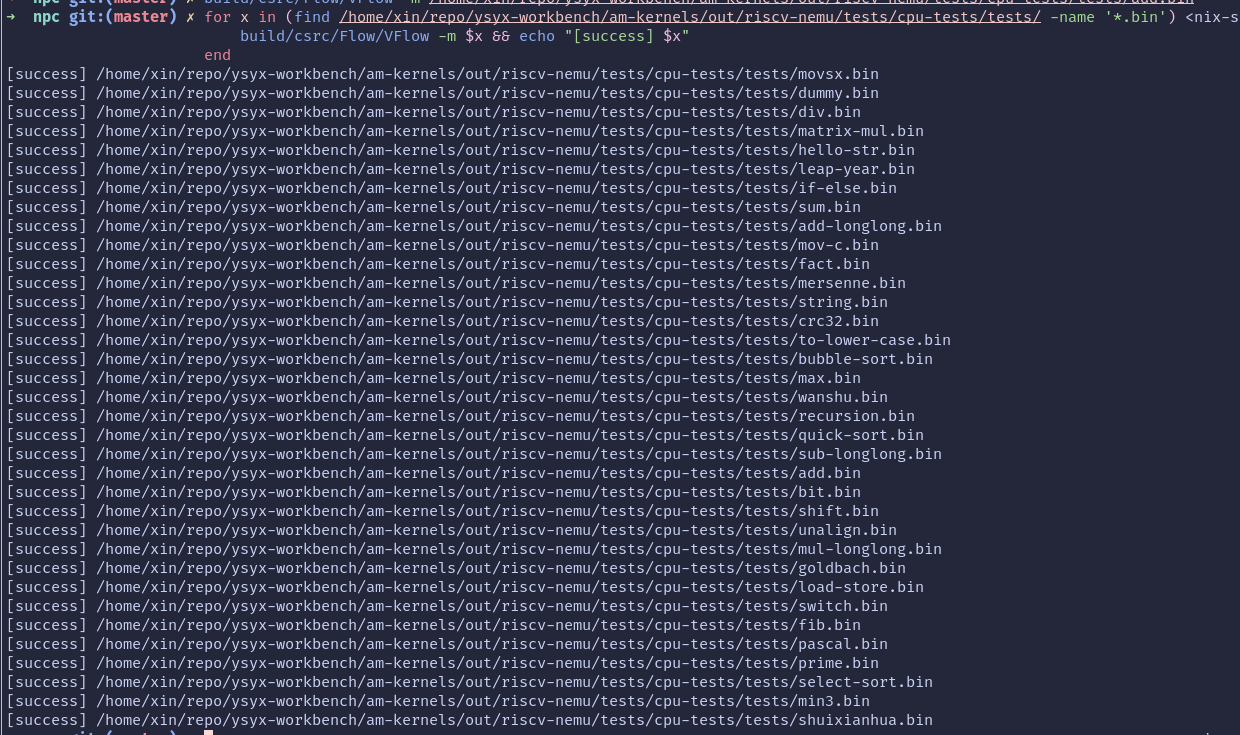
\includegraphics[width=\textwidth]{resources/test-cpu.png}
    \subcaption{cpu-tests测试结果}
    \label{fig:test-cpu}
\end{figure}

\begin{figure}
\centering

\begin{minipage}[t]{0.45\textwidth}
    \centering
    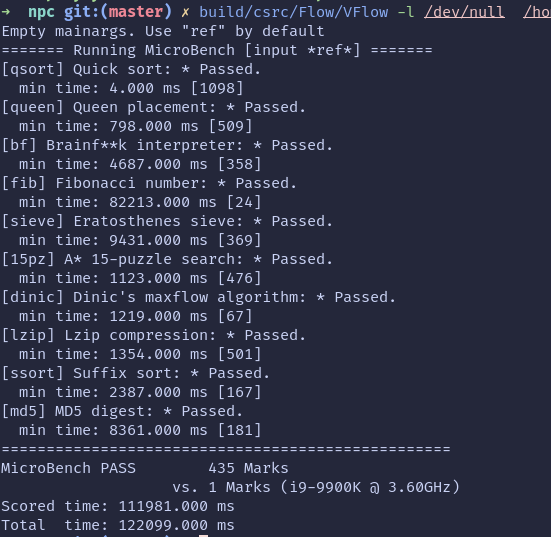
\includegraphics[width=\textwidth]{resources/test-bench.png}
    \subcaption{microbench测试结果}
    \label{fig:test-bench}
\end{minipage}
\begin{minipage}[t]{0.45\textwidth}
    \centering
    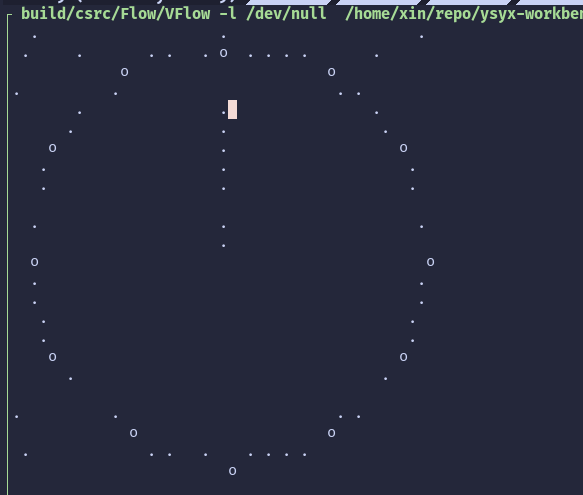
\includegraphics[width=\textwidth]{resources/test-clock.png}
    \subcaption{demo程序运行结果}
    \label{fig:2-machines-bm}
\end{minipage}
\caption{microbench和demo运行结果}
\end{figure}

\section{持续测试平台的搭建}

为了能够在芯片迭代的过程中持续对芯片的功能和性能进行测试,本文还搭建了持续测试平台。每次提交代码时,测试都会自动编译、测试,并报告可能发生的错误。

测试平台基于Gitea action搭建,可以离线部署,后续可以添加自动判分的功能,从而实现在课堂实验上使用。

\begin{figure}
    \centering
    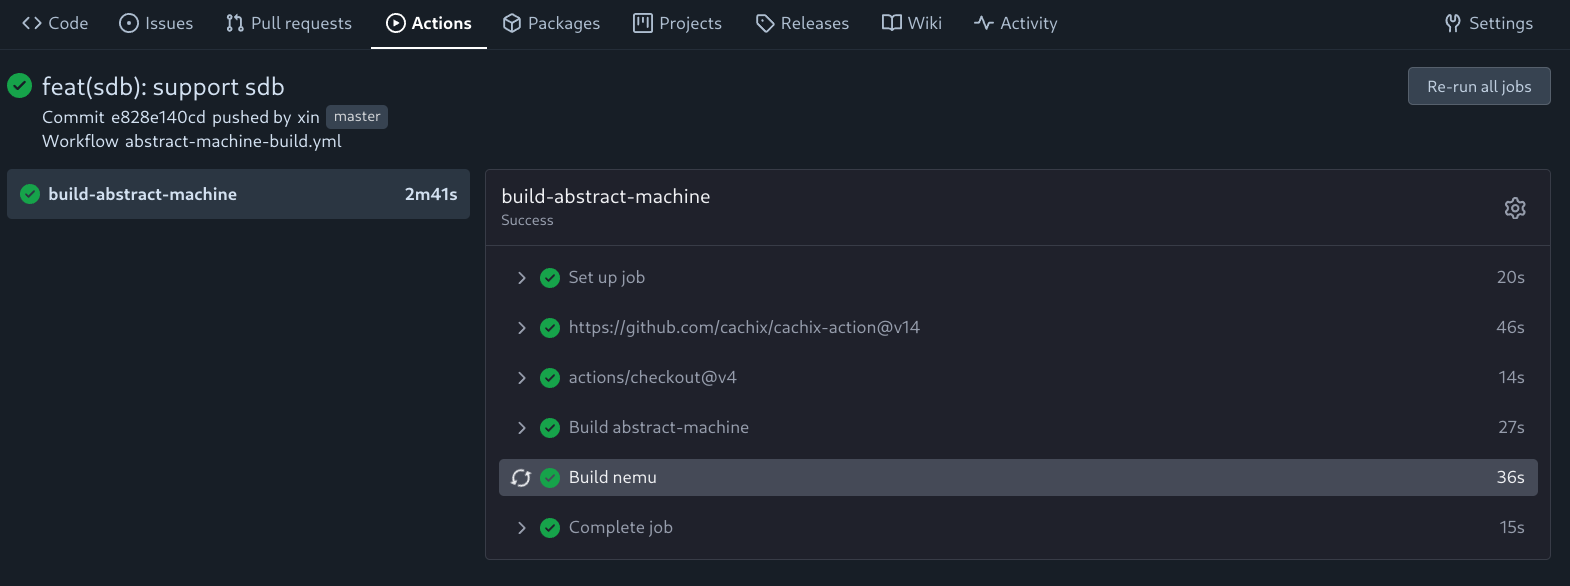
\includegraphics[width=0.8\textwidth]{resources/test-ci.png}
    \caption{持续测试平台运行}
    \label{fig:test-ci}
\end{figure}

